
\section{Introduction\label{introduction}}

Automatic knowledge base construction (AKBC) is the task of building a structured knowledge base (KB) of facts using raw text evidence, and often an initial seed KB to be augmented~\citep{NELL,yago,freebase}.
Extracted facts about entities and their relations are useful for many downsteam tasks such as question answering, query understanding, etc.
An effective approach to AKBC is Universal Schema.
Universal Schema embeds textual patters and knowledge bases into a shared space in order to reason over relations and entity pairs.
A low dimensional embedding is learned for each entity pair and each relation type using matrix factorization.
The model is then able to infer relations between entities as the dot product between the two entity pair and relation type vectors.

Unfortunately, this formulation limits the generalization of the model.
In its original form, Universal Schema can only reason about entity pairs and textual relations explicitly seen at training time.
In this work we extend Universal Schema to represent entity pairs not as a learned dense vector representation, but as an aggregate function over its relation types.
This allows Universal Schema to form predictions for all entity pairs - whether seen in training or not - and makes a direct connection between the prediction and its provenance.
% this is breaking compilation
%We demonstrate that our relation only models perform competitively with models using explicit entity pair vectors.



\section {Background}

\subsection {Universal Schema}
The Universal Schema \citep{limin} approach to AKBC jointly embeds any number of KB and text corpara into a shared embedded space to jointly reason over entities and their relations (See figure \ref {fig:uschema-matrix}).

\citet{limin} proposed several model variants operating on entities and entity pairs and other extensions have been proposed \citep{yao2013universal,vector_pra,neelakantan2015compositional,logicmfnaacl15}. Recently, Universal Schema has been extended to deal with compositional representations of textual relations \citep{toutanova2015representing,verga2015multilingual} allowing it to generalize to all possible textual patterns and reason over any arbitrary text.

\begin{figure}[h]
\caption{Universal schema represents relation types and entity pairs as a matrix.
1's are observed training examples and the bolded .93 is predicted by the model.
\label{fig:uschema-matrix}}
\centering
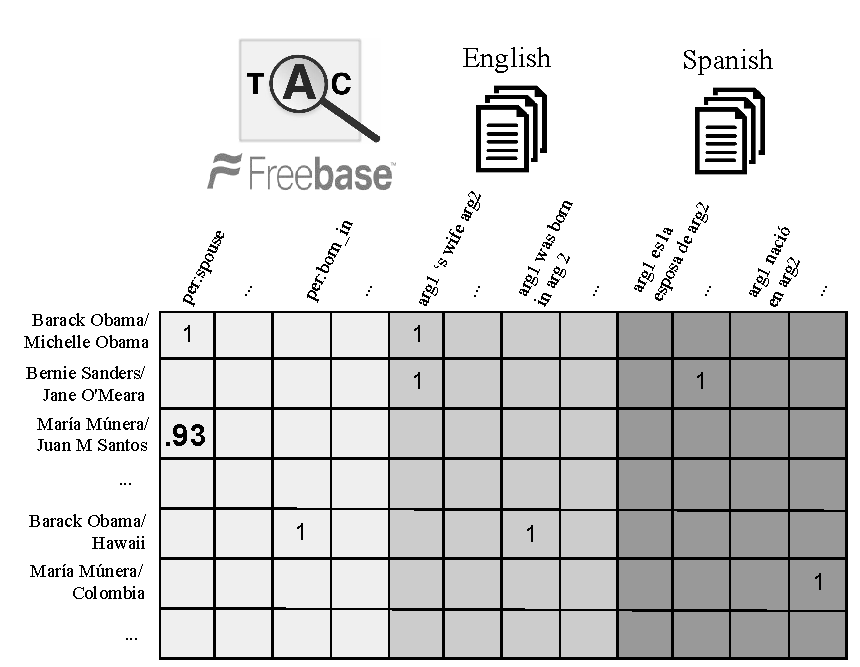
\includegraphics[scale=.68]{matrix}
\end{figure}



\subsection {Entities vs Entity Pairs}

A knowledge base is naturally described as a graph, in which entities are nodes and relations are labeled edges~\citep{yago,freebase}.
In the case of \emph{knowledge graph completion}, the task is akin to link prediction, assuming an initial set of (\emph{s, r, o}) triples.
See~\citet{nickel2015review} for a review.
No accompanying text data is necessary, since links can be predicted using properties of the graph, such as transitivity.
In order to generalize well, prediction is often posed as low-rank matrix or tensor factorization.
A variety of model variants have been suggested, where the probability of a given edge existing depends on a multi-linear form~\citep{rescal,DBLP:journals/corr/Garcia-DuranBUG15,bishan,transe,wang2014knowledge,lin2015learning}, or non-linear interactions between $s$, $r$, and $o$~\citep{socherkb}.

These models all operate at the level of entities rather than entity pairs.
Entity-based models have recall advantages over entity pairs.
For any two entities, the model is able to make predictions even if there is no information regarding the explicit entity pair.
However, this essentially reduces to type clustering.

Entity pairs on the other hand have higher precision.
Both~\citet{toutanova2015representing} and~\citet{limin} observed that the entity pair model outperforms entity models in cases where the entity pair was seen at training time.
This is particularly important when jointly embedding text and knowledge bases.
By leveraging large amounts of unlabeled text, Universal Schema is able to find additional textual evidence for entity pairs.
We are interested in high precision information extraction from direct textual provenance.

Universal Schema models entity pairs  as an explicit vector.
We instead treat each entity pair as an aggregate function over each of its relation types.
This allows us to trivially extend to unseen entity pairs, have a direct link to provenance, and allocate a variable number of parameters per entity pair.


%\subsection {Compositional Universal Schema}
%
%Recently, Universal Schema has been extended to deal with compositional representations of textual relations \citep{toutanova2015representing,verga2015multilingual}.
%
%Compositional Universal Schema has two main advantages over explicit modeling of textual patterns.
%The first is that it allows for the model to share statistics between very similar patterns.
%Instead of modeling the text pattern 'lives in the city' and 'lives in the city of' as distinct atomic units, they can instead be composed compositionally of the same word embeddings.
%Second, and even more importantly, Compositional Universal Schema allows us to generalize to all possible textual patterns, allowing us to reason over any arbitrary text.

%\begin{figure}[h]
%\caption{Top : Universal Schema expresses each textual pattern as an atomic unit \protect\citet{riedel2010modeling}.
%Bottom : Compositional Universal Schema uses an lstm to encode each textual relation \protect\cite{verga2015multilingual}. }
%\centering
%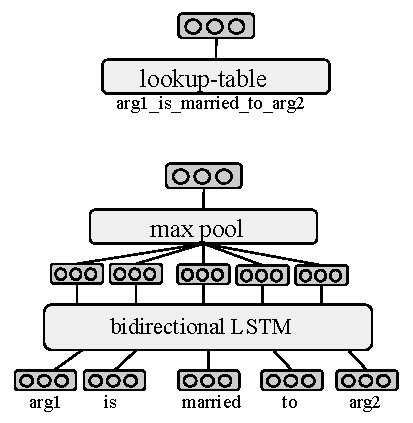
\includegraphics[scale=.68]{relation-models}
%\end{figure}

